\documentclass[12pt,a4paper]{article}

\usepackage[utf8]{inputenc}
\usepackage[T2A]{fontenc}
\usepackage[ukrainian]{babel}

\usepackage{geometry}
\geometry{left=2cm,right=2cm,top=2cm,bottom=2cm}

\usepackage{graphicx}
\usepackage{array,multirow}
\usepackage{booktabs}
\usepackage{caption}

\usepackage{tcolorbox}

\renewcommand{\thetable}{№\arabic{table}}
\captionsetup[table]{name=Таблиця}

\usepackage{amsmath}
\usepackage{pdflscape}
\usepackage{xcolor}

\usepackage{fvextra}
\usepackage{upquote}

\usepackage{hyperref}

\usepackage{minted}

\usemintedstyle{vs}
\setminted{linenos, breaklines, frame=single, fontsize=\small}

\RecustomVerbatimCommand{\VerbatimInput}{VerbatimInput}{
    breaklines=true,
    breaksymbolleft={}
}

% Узагальнений стиль для коду
\newminted{java}{
  fontsize=\small,
  baselinestretch=1.05,
  breaklines,
  linenos,
  frame=lines,
  framesep=2mm
}

% Консоль/PowerShell як plain text
\newminted{text}{
  fontsize=\small,
  breaklines,
  frame=single,
  bgcolor=gray!5
}

\begin{document}

    \begin{titlepage}

        % Картинка шапки (по центру, з відступом від верху)
        \begin{center}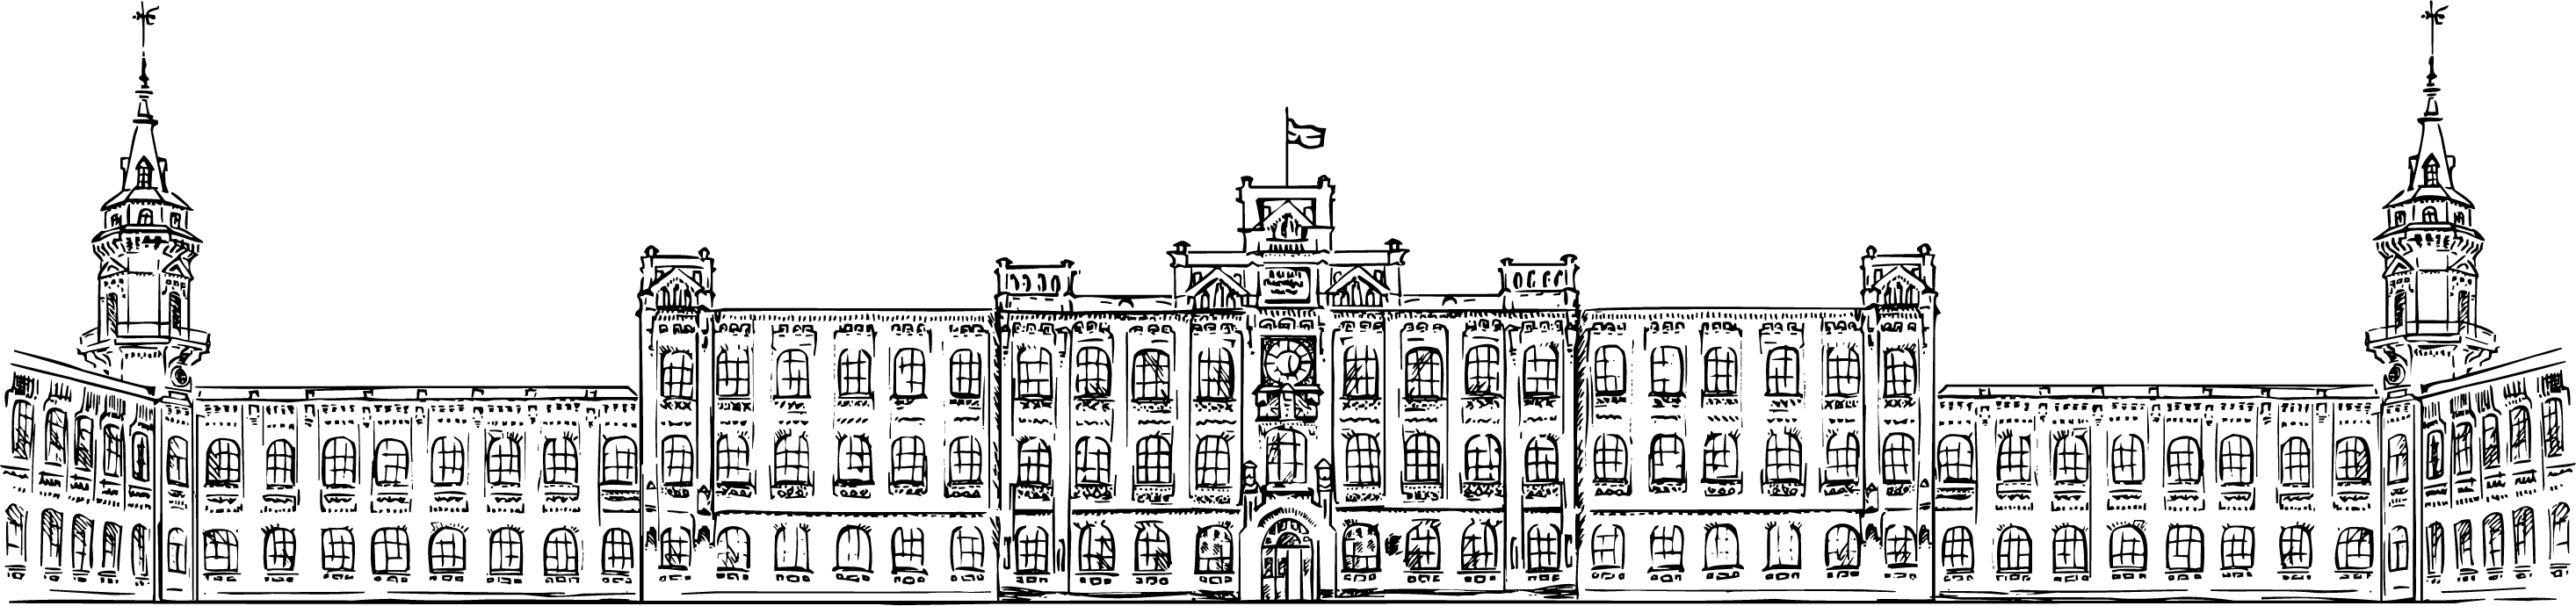
\includegraphics[width=0.7\textwidth]{../../../TITLES/letterhead.png}\end{center}

        \begin{center}
            \large Національний технічний університет України\\
            «Київський політехнічний інститут імені Ігоря Сікорського»\\[1em]
            Факультет інформатики та обчислювальної техніки\\
            Кафедра обчислювальної техніки
        \end{center}

        \vfill

        \begin{center}
            \textbf{\LARGE Інженерія програмного забезпечення}\\[2em]
            \textbf{\Large Практична робота №3}\\[0.5em]
            «Структурні шаблони проектування ПЗ. Composite, Decorator, Proxy, Flyweight, Adapter, Bridge, Facade»
        \end{center}

        \vfill

        \begin{flushright}
            Виконав: студент 2 курсу ФІОТ, гр. ІО-41\\
            \textit{Давидчук А.~М.}\\
            Залікова книжка № 4106\\[1em]
            Перевірив: \textit{Васильєва М.~Д.}
        \end{flushright}

        \vfill

        \begin{center}Київ --- 2025\end{center}

    \end{titlepage}

    % Основний документ:

    \setlength{\parindent}{0em}

    \textbf{\underline{Тема:}} «Структурні шаблони проектування ПЗ. Composite, Decorator, Proxy, Flyweight, Adapter, Bridge, Facade».
    
    \vspace{1em}

    \textbf{\underline{Мета:}} Ознайомлення з видами шаблонів проектування ПЗ. Вивчення структурних
    шаблонів. Отримання базових навичок з застосування шаблонів Composite, Decorator, Proxy,
    Flyweight, Adapter, Bridge, Facade.

    \begin{center} \textbf{\Large Практична частина (Завдання №1)} \end{center}

    \setlength{\parindent}{1.5em}

    Мій номер залікової книги: $4106$, звідси $4106 \text{ mod } 12 = 2$. Тому умова до 2 завдання буде:

    Клас \texttt{GameElement}, який представляє елемент ігрового простору.

    Необхідно розширити функціональність так, щоб:
    \begin{itemize}
        \item Можна було створювати простий елемент (наприклад, одиночний об'єкт на рівні).
        \item Кожний елемент мав розмір (ширина та висота) у умовних одиницях.
        \item Можна було створювати композитний елемент (групу елементів), у якому:
        \begin{itemize}
            \item Атрибути розміру та площа обчислюються динамічно на основі вкладених елементів.
            \item Можливі вкладені композитні елементи (багаторівнева ієрархія).
        \end{itemize}
        \item Можна було отримати площу елемента:
        \begin{itemize}
            \item Для простого елемента – площа = ширина × висота.
            \item Для композитного елемента – площа = сума площ усіх вкладених елементів або мінімальна обгортка, що охоплює всі піделементи (залежно від реалізації).
        \end{itemize}
    \end{itemize}

    \textbf{Вимоги}
    \begin{itemize}
        \item Не змінювати існуючий клас \texttt{GameElement}. Реалізувати можливість гнучкого додавання нових типів елементів у майбутньому.
        \item Продемонструвати у методі \texttt{main} кілька варіантів роботи з елементами:
        \begin{itemize}
            \item окремий простий елемент,
            \item група з кількох простих елементів,
            \item група з вкладеними групами (багаторівнева структура).
        \end{itemize}
    \end{itemize}

    \setlength{\parindent}{0em}

    \textbf{\underline{Загальна структура проекту до компіляції:}}

    \begin{minted}{text}
PS C:\Users\Artem Davydchuk\Desktop\reps\university_roadmap\semestr3\software engineering\labs\lab3\project1> tree /f /a
Folder PATH listing
Volume serial number is 9873-FF92
C:.
|   build.xml
|
\---src
        AreaMode.java
        CompositeElement.java
        IGameElement.java
        Main.java
        SimpleElement.java
    \end{minted}

    \textbf{\underline{Код build.xml задля автоматизації:}}

    \begin{minted}{xml}
<?xml version="1.0" encoding="UTF-8"?>
<project name="lab3: First Task" default="all" basedir=".">

  <!-- ===== Properties ===== -->
  <property name="src.dir"      value="src"/>
  <property name="build.dir"    value="out"/>
  <property name="classes.dir"  value="${build.dir}"/>
  <property name="doc.dir"      value="doc"/>
  <property name="main.class"   value="Main"/>
  <property name="java.release" value="17"/>

  <!-- ===== Clean ===== -->
  <target name="clean" description="Remove compiled classes and docs">
    <delete dir="${build.dir}"/>
    <delete dir="${doc.dir}"/>
  </target>

  <!-- ===== Compile ===== -->
  <target name="compile" description="Compile sources" depends="prepare">
    <mkdir dir="${classes.dir}"/>
    <javac srcdir="${src.dir}"
           destdir="${classes.dir}"
           includeantruntime="false"
           debug="true"
           encoding="UTF-8"
           release="${java.release}">
      <include name="**/*.java"/>
    </javac>
  </target>

  <target name="prepare">
    <mkdir dir="${classes.dir}"/>
  </target>

  <!-- ===== Run ===== -->
  <target name="run" description="Run main class" depends="compile">
    <java classname="${main.class}" fork="true" failonerror="true">
      <classpath>
        <path location="${classes.dir}"/>
      </classpath>
    </java>
  </target>

  <!-- ===== Javadoc ===== -->
  <target name="javadoc" description="Generate Javadoc">
    <mkdir dir="${doc.dir}"/>
    <javadoc destdir="${doc.dir}"
             sourcepath="${src.dir}"
             encoding="UTF-8"
             author="true"
             version="true"
             use="true"
             windowtitle="Composite Pattern — Lab 3 API"
             doctitle="Composite Pattern — Lab 3 API"
             failonerror="false">
      <fileset dir="${src.dir}">
        <include name="**/*.java"/>
      </fileset>
      <link href="https://docs.oracle.com/en/java/javase/${java.release}/docs/api/"/>
    </javadoc>
  </target>

  <!-- ===== Convenience: all-in-one ===== -->
  <target name="all" description="Clean, compile, run, and generate Javadoc"
          depends="clean,compile,run,javadoc"/>
</project>
    \end{minted}

    \textbf{\underline{Функціонал (таргети), який реалізує \texttt{build.xml}}}

    \begin{minted}{text}
Buildfile: C:\Users\Artem Davydchuk\Desktop\reps\university_roadmap\semestr3\software engineering\labs\lab3\project1\build.xml

Main targets:

 all      Clean, compile, run, and generate Javadoc
 clean    Remove compiled classes and docs
 compile  Compile sources
 javadoc  Generate Javadoc
 run      Run main class
Default target: all
    \end{minted}

    \textbf{\underline{Код \texttt{AreaMode.java}:}}

    \begin{minted}{java}
/**
 * Area calculation modes for a composite element.
 */
public enum AreaMode {
    /** Area equals the sum of all child areas. */
    SUM_CHILD_AREAS,

    /** Area equals the area of the minimal bounding box covering all children. */
    BOUNDING_BOX
}
    \end{minted}

    \textbf{\underline{Код \texttt{CompositeElement.java}:}}

    \begin{minted}{java}
import java.util.ArrayList;
import java.util.List;

/**
 * Composite element (group) in the {@code Composite} pattern.
 * <p>
 * Holds child elements, supports nested composites, and computes size dynamically
 * from children. Area calculation is configurable via {@link AreaMode}.
 */
public class CompositeElement implements IGameElement {
    private final String name;
    private int x, y; // local position in the parent
    private final List<IGameElement> children = new ArrayList<>();
    private AreaMode areaMode = AreaMode.SUM_CHILD_AREAS;

    /**
     * Creates a composite with a human-readable name.
     * @param name composite name
     */
    public CompositeElement(String name) { this.name = name; }

    /**
     * Sets the area calculation mode.
     * @param mode mode to use
     * @return this composite (for fluent chaining)
     */
    public CompositeElement setAreaMode(AreaMode mode) {
        this.areaMode = mode;
        return this;
    }

    /**
     * Adds a child at the given local position within this composite.
     * @param child       element to add (simple or composite)
     * @param childLocalX child local X
     * @param childLocalY child local Y
     */
    public void add(IGameElement child, int childLocalX, int childLocalY) {
        child.setPosition(childLocalX, childLocalY);
        children.add(child);
    }

    /**
     * Removes the given child if present.
     * @param child child to remove
     */
    public void remove(IGameElement child) {
        children.remove(child);
    }

    /**
     * @return internal list of children (treat as read-only)
     */
    public List<IGameElement> getChildren() { return children; }

    /** {@inheritDoc} */
    @Override public String name() { return name; }

    /** {@inheritDoc} */
    @Override public int getX() { return x; }

    /** {@inheritDoc} */
    @Override public int getY() { return y; }

    /** {@inheritDoc} */
    @Override public void setPosition(int x, int y) { this.x = x; this.y = y; }

    /**
     * Computes width as the width of the minimal bounding box enclosing all children.
     * Empty composite has width 0.
     */
    @Override
    public int getWidth() {
        if (children.isEmpty()) return 0;
        int minX = Integer.MAX_VALUE, maxX = Integer.MIN_VALUE;
        for (var c : children) {
            int left = c.getX();
            int right = c.getX() + c.getWidth();
            minX = Math.min(minX, left);
            maxX = Math.max(maxX, right);
        }
        return Math.max(0, maxX - minX);
    }

    /**
     * Computes height as the height of the minimal bounding box enclosing all children.
     * Empty composite has height 0.
     */
    @Override
    public int getHeight() {
        if (children.isEmpty()) return 0;
        int minY = Integer.MAX_VALUE, maxY = Integer.MIN_VALUE;
        for (var c : children) {
            int top = c.getY();
            int bottom = c.getY() + c.getHeight();
            minY = Math.min(minY, top);
            maxY = Math.max(maxY, bottom);
        }
        return Math.max(0, maxY - minY);
    }

    /**
     * Computes area according to {@link AreaMode}.
     * SUM_CHILD_AREAS: sum of child areas.
     * BOUNDING_BOX: getWidth() * getHeight().
     */
    @Override
    public int area() {
        if (areaMode == AreaMode.SUM_CHILD_AREAS) {
            int sum = 0;
            for (var c : children) sum += c.area();
            return sum;
        } else {
            return getWidth() * getHeight();
        }
    }

    /** {@inheritDoc} */
    @Override
    public void draw(int x, int y) {
        int absX = x + this.x;
        int absY = y + this.y;
        System.out.printf(
            "Composite.draw name=%s at=(%d,%d) size=%dx%d mode=%s children=%d%n",
            name, absX, absY, getWidth(), getHeight(), areaMode, children.size()
        );
        for (var c : children) c.draw(absX, absY);
    }
}
    \end{minted}

    \textbf{\underline{Код \texttt{IGameElement.java}:}}

    \begin{minted}{java}
/**
 * Base interface for an element of the game space.
 * <p>
 * Serves as the <b>Component</b> role in the <em>Composite</em> pattern,
 * defining a common contract for both simple and composite elements.
 */
public interface IGameElement {

    /** @return human-readable name (for logs/debugging) */
    String name();

    /** @return local X coordinate within parent composite */
    int getX();

    /** @return local Y coordinate within parent composite */
    int getY();

    /**
     * Sets the local position of this element relative to its parent composite.
     * @param x local X
     * @param y local Y
     */
    void setPosition(int x, int y);

    /**
     * Width of the element.
     * For composites, this is computed dynamically from the children's bounding box.
     * @return non-negative width
     */
    int getWidth();

    /**
     * Height of the element.
     * For composites, this is computed dynamically from the children's bounding box.
     * @return non-negative height
     */
    int getHeight();

    /**
     * Area of the element.
     * For composites, the calculation depends on {@link AreaMode}.
     * @return non-negative area
     */
    int area();

    /**
     * Demonstrational business method (drawing/logging).
     * Should print an informative line to the console.
     * @param x absolute X coordinate of the parent origin
     * @param y absolute Y coordinate of the parent origin
     */
    void draw(int x, int y);
}
    \end{minted}

    \textbf{\underline{Код \texttt{SimpleElement.java}:}}

    \begin{minted}{java}
/**
 * Leaf element in the {@code Composite} pattern.
 * <p>
 * Represents an indivisible game object with fixed size
 * (width × height) and a local position within its parent composite.
 */
public class SimpleElement implements IGameElement {
    private final String name;
    private int x, y;          // local position in parent
    private final int width;
    private final int height;

    /**
     * Creates a simple element with given name and size.
     * Negative width/height are clamped to zero.
     *
     * @param name   element name (for logs/debugging)
     * @param width  width (non-negative)
     * @param height height (non-negative)
     */
    public SimpleElement(String name, int width, int height) {
        this.name = name;
        this.width = Math.max(0, width);
        this.height = Math.max(0, height);
    }

    /** {@inheritDoc} */
    @Override public String name() { return name; }

    /** {@inheritDoc} */
    @Override public int getX() { return x; }

    /** {@inheritDoc} */
    @Override public int getY() { return y; }

    /** {@inheritDoc} */
    @Override public void setPosition(int x, int y) { this.x = x; this.y = y; }

    /** {@inheritDoc} */
    @Override public int getWidth() { return width; }

    /** {@inheritDoc} */
    @Override public int getHeight() { return height; }

    /** {@inheritDoc} */
    @Override public int area() { return width * height; }

    /** {@inheritDoc} */
    @Override
    public void draw(int x, int y) {
        System.out.printf("Simple.draw name=%s at=(%d,%d) size=%dx%d%n",
                name, x + this.x, y + this.y, width, height);
    }
}
    \end{minted}

    \textbf{\underline{Код \texttt{Main.java}:}}

    \begin{minted}{java}
/**
 * Demo/Client that showcases the Composite pattern implementation
 * with three scenarios required by the lab:
 * <ol>
 *   <li>single simple element;</li>
 *   <li>composite with several simple elements;</li>
 *   <li>nested composite structure (composite inside composite)
 *       and different area modes.</li>
 * </ol>
 */
public class Main {
    /**
     * Program entry point.
     * @param args unused
     */
    public static void main(String[] args) {
        // 1) Single simple element
        IGameElement hero = new SimpleElement("Hero", 2, 3);
        hero.setPosition(5, 7);
        hero.draw(0, 0);
        System.out.printf("Hero area=%d size=%dx%d%n%n", hero.area(), hero.getWidth(), hero.getHeight());

        // 2) Composite with several simple elements (area mode: SUM_CHILD_AREAS)
        CompositeElement group1 = new CompositeElement("Group1").setAreaMode(AreaMode.SUM_CHILD_AREAS);
        group1.add(new SimpleElement("Tree", 3, 4), 0, 0);
        group1.add(new SimpleElement("Rock", 2, 2), 4, 1);
        group1.add(new SimpleElement("Chest", 1, 1), 7, 0);
        group1.setPosition(10, 10);
        group1.draw(0, 0);
        System.out.printf("Group1 area=%d size=%dx%d%n%n", group1.area(), group1.getWidth(), group1.getHeight());

        // 3) Nested composite (outer uses BOUNDING_BOX, inner uses SUM_CHILD_AREAS)
        CompositeElement inner = new CompositeElement("Inner").setAreaMode(AreaMode.SUM_CHILD_AREAS);
        inner.add(new SimpleElement("Coin", 1, 1), 1, 0);
        inner.add(new SimpleElement("Key",  1, 2), 2, 2);

        CompositeElement outer = new CompositeElement("Outer").setAreaMode(AreaMode.BOUNDING_BOX);
        outer.add(new SimpleElement("Door", 2, 5), 0, 0);
        outer.add(inner, 5, 1);
        outer.setPosition(20, 3);

        outer.draw(0, 0);
        System.out.printf("Outer area(mode=%s)=%d size=%dx%d%n",
                AreaMode.BOUNDING_BOX, outer.area(), outer.getWidth(), outer.getHeight());
    }
}
    \end{minted}

    \textbf{\underline{Результат виконання команди \texttt{all}:}}

    \begin{minted}{text}
PS C:\Users\Artem Davydchuk\Desktop\reps\university_roadmap\semestr3\software engineering\labs\lab3\project1> ant all
Buildfile: C:\Users\Artem Davydchuk\Desktop\reps\university_roadmap\semestr3\software engineering\labs\lab3\project1\build.xml

clean:

prepare:
    [mkdir] Created dir: C:\Users\Artem Davydchuk\Desktop\reps\university_roadmap\semestr3\software engineering\labs\lab3\project1\out

compile:
    [javac] Compiling 5 source files to C:\Users\Artem Davydchuk\Desktop\reps\university_roadmap\semestr3\software engineering\labs\lab3\project1\out

run:
     [java] Simple.draw name=Hero at=(5,7) size=2x3
     [java] Hero area=6 size=2x3
     [java]
     [java] Composite.draw name=Group1 at=(10,10) size=8x4 mode=SUM_CHILD_AREAS children=3
     [java] Simple.draw name=Tree at=(10,10) size=3x4
     [java] Simple.draw name=Rock at=(14,11) size=2x2
     [java] Simple.draw name=Chest at=(17,10) size=1x1
     [java] Group1 area=17 size=8x4
     [java]
     [java] Composite.draw name=Outer at=(20,3) size=7x5 mode=BOUNDING_BOX children=2
     [java] Simple.draw name=Door at=(20,3) size=2x5
     [java] Composite.draw name=Inner at=(25,4) size=2x4 mode=SUM_CHILD_AREAS children=2
     [java] Simple.draw name=Coin at=(26,4) size=1x1
     [java] Simple.draw name=Key at=(27,6) size=1x2
     [java] Outer area(mode=BOUNDING_BOX)=35 size=7x5

javadoc:
    [mkdir] Created dir: C:\Users\Artem Davydchuk\Desktop\reps\university_roadmap\semestr3\software engineering\labs\lab3\project1\doc
  [javadoc] C:\Users\Artem Davydchuk\Desktop\reps\university_roadmap\semestr3\software engineering\labs\lab3\project1\src contains source files in the default package, you must specify them as source files not packages.
  [javadoc] Generating Javadoc
  [javadoc] Javadoc execution
  [javadoc] Loading source file C:\Users\Artem Davydchuk\Desktop\reps\university_roadmap\semestr3\software engineering\labs\lab3\project1\src\AreaMode.java...
  [javadoc] Loading source file C:\Users\Artem Davydchuk\Desktop\reps\university_roadmap\semestr3\software engineering\labs\lab3\project1\src\CompositeElement.java...
  [javadoc] Loading source file C:\Users\Artem Davydchuk\Desktop\reps\university_roadmap\semestr3\software engineering\labs\lab3\project1\src\IGameElement.java...
  [javadoc] Loading source file C:\Users\Artem Davydchuk\Desktop\reps\university_roadmap\semestr3\software engineering\labs\lab3\project1\src\Main.java...
  [javadoc] Loading source file C:\Users\Artem Davydchuk\Desktop\reps\university_roadmap\semestr3\software engineering\labs\lab3\project1\src\SimpleElement.java...
  [javadoc] Constructing Javadoc information...
  [javadoc] Building index for all the packages and classes...
  [javadoc] Standard Doclet version 21.0.8+12-LTS-250
  [javadoc] Building tree for all the packages and classes...
  [javadoc] Generating C:\Users\Artem Davydchuk\Desktop\reps\university_roadmap\semestr3\software engineering\labs\lab3\project1\doc\AreaMode.html...
  [javadoc] Generating C:\Users\Artem Davydchuk\Desktop\reps\university_roadmap\semestr3\software engineering\labs\lab3\project1\doc\CompositeElement.html...
  [javadoc] C:\Users\Artem Davydchuk\Desktop\reps\university_roadmap\semestr3\software engineering\labs\lab3\project1\src\IGameElement.java:9: warning: no main description
  [javadoc]     /** @return human-readable name (for logs/debugging) */
  [javadoc]         ^
  [javadoc] C:\Users\Artem Davydchuk\Desktop\reps\university_roadmap\semestr3\software engineering\labs\lab3\project1\src\IGameElement.java:12: warning: no main description
  [javadoc]     /** @return local X coordinate within parent composite */
  [javadoc]         ^
  [javadoc] C:\Users\Artem Davydchuk\Desktop\reps\university_roadmap\semestr3\software engineering\labs\lab3\project1\src\IGameElement.java:15: warning: no main description
  [javadoc]     /** @return local Y coordinate within parent composite */
  [javadoc]         ^
  [javadoc] C:\Users\Artem Davydchuk\Desktop\reps\university_roadmap\semestr3\software engineering\labs\lab3\project1\src\CompositeElement.java:52: warning: no main description
  [javadoc]      * @return internal list of children (treat as read-only)
  [javadoc]        ^
  [javadoc] Generating C:\Users\Artem Davydchuk\Desktop\reps\university_roadmap\semestr3\software engineering\labs\lab3\project1\doc\IGameElement.html...
  [javadoc] Generating C:\Users\Artem Davydchuk\Desktop\reps\university_roadmap\semestr3\software engineering\labs\lab3\project1\doc\Main.html...
  [javadoc] C:\Users\Artem Davydchuk\Desktop\reps\university_roadmap\semestr3\software engineering\labs\lab3\project1\src\Main.java:11: warning: use of default constructor, which does not provide a comment
  [javadoc] public class Main {
  [javadoc]        ^
  [javadoc] Generating C:\Users\Artem Davydchuk\Desktop\reps\university_roadmap\semestr3\software engineering\labs\lab3\project1\doc\SimpleElement.html...
  [javadoc] Generating C:\Users\Artem Davydchuk\Desktop\reps\university_roadmap\semestr3\software engineering\labs\lab3\project1\doc\package-summary.html...
  [javadoc] Generating C:\Users\Artem Davydchuk\Desktop\reps\university_roadmap\semestr3\software engineering\labs\lab3\project1\doc\package-tree.html...
  [javadoc] Generating C:\Users\Artem Davydchuk\Desktop\reps\university_roadmap\semestr3\software engineering\labs\lab3\project1\doc\class-use\AreaMode.html...
  [javadoc] Generating C:\Users\Artem Davydchuk\Desktop\reps\university_roadmap\semestr3\software engineering\labs\lab3\project1\doc\class-use\CompositeElement.html...
  [javadoc] Generating C:\Users\Artem Davydchuk\Desktop\reps\university_roadmap\semestr3\software engineering\labs\lab3\project1\doc\class-use\IGameElement.html...
  [javadoc] Generating C:\Users\Artem Davydchuk\Desktop\reps\university_roadmap\semestr3\software engineering\labs\lab3\project1\doc\class-use\Main.html...
  [javadoc] Generating C:\Users\Artem Davydchuk\Desktop\reps\university_roadmap\semestr3\software engineering\labs\lab3\project1\doc\class-use\SimpleElement.html...
  [javadoc] Generating C:\Users\Artem Davydchuk\Desktop\reps\university_roadmap\semestr3\software engineering\labs\lab3\project1\doc\package-use.html...
  [javadoc] Generating C:\Users\Artem Davydchuk\Desktop\reps\university_roadmap\semestr3\software engineering\labs\lab3\project1\doc\overview-tree.html...
  [javadoc] Building index for all classes...
  [javadoc] Generating C:\Users\Artem Davydchuk\Desktop\reps\university_roadmap\semestr3\software engineering\labs\lab3\project1\doc\allclasses-index.html...
  [javadoc] Generating C:\Users\Artem Davydchuk\Desktop\reps\university_roadmap\semestr3\software engineering\labs\lab3\project1\doc\allpackages-index.html...
  [javadoc] Generating C:\Users\Artem Davydchuk\Desktop\reps\university_roadmap\semestr3\software engineering\labs\lab3\project1\doc\index-all.html...
  [javadoc] Generating C:\Users\Artem Davydchuk\Desktop\reps\university_roadmap\semestr3\software engineering\labs\lab3\project1\doc\search.html...
  [javadoc] Generating C:\Users\Artem Davydchuk\Desktop\reps\university_roadmap\semestr3\software engineering\labs\lab3\project1\doc\index.html...
  [javadoc] Generating C:\Users\Artem Davydchuk\Desktop\reps\university_roadmap\semestr3\software engineering\labs\lab3\project1\doc\help-doc.html...
  [javadoc] 5 warnings

all:

BUILD SUCCESSFUL
Total time: 5 seconds
    \end{minted}

    \textbf{\underline{Оновлене дерево робочої директорії:}}

    \begin{minted}{text}
PS C:\Users\Artem Davydchuk\Desktop\reps\university_roadmap\semestr3\software engineering\labs\lab3\project1> tree /f /a
Folder PATH listing
Volume serial number is 9873-FF92
C:.
|   build.xml
|
+---doc
|   |   allclasses-index.html
|   |   allpackages-index.html
|   |   AreaMode.html
|   |   CompositeElement.html
|   |   copy.svg
|   |   element-list
|   |   help-doc.html
|   |   IGameElement.html
|   |   index-all.html
|   |   index.html
|   |   link.svg
|   |   Main.html
|   |   member-search-index.js
|   |   module-search-index.js
|   |   overview-tree.html
|   |   package-search-index.js
|   |   package-summary.html
|   |   package-tree.html
|   |   package-use.html
|   |   script.js
|   |   search-page.js
|   |   search.html
|   |   search.js
|   |   SimpleElement.html
|   |   stylesheet.css
|   |   tag-search-index.js
|   |   type-search-index.js
|   |
|   +---class-use
|   |       AreaMode.html
|   |       CompositeElement.html
|   |       IGameElement.html
|   |       Main.html
|   |       SimpleElement.html
|   |
|   +---legal
|   |       COPYRIGHT
|   |       jquery.md
|   |       jqueryUI.md
|   |       LICENSE
|   |
|   +---resources
|   |       glass.png
|   |       x.png
|   |
|   \---script-dir
|           jquery-3.7.1.min.js
|           jquery-ui.min.css
|           jquery-ui.min.js
|
+---out
|       AreaMode.class
|       CompositeElement.class
|       IGameElement.class
|       Main.class
|       SimpleElement.class
|
\---src
        AreaMode.java
        CompositeElement.java
        IGameElement.java
        Main.java
        SimpleElement.java
    \end{minted}

    \newpage

    \textbf{\underline{Додатковий окремий запуск Main:}}

    \begin{minted}{text}
PS C:\Users\Artem Davydchuk\Desktop\reps\university_roadmap\semestr3\software engineering\labs\lab3\project1> java -cp out Main
Simple.draw name=Hero at=(5,7) size=2x3
Hero area=6 size=2x3

Composite.draw name=Group1 at=(10,10) size=8x4 mode=SUM_CHILD_AREAS children=3
Simple.draw name=Tree at=(10,10) size=3x4
Simple.draw name=Rock at=(14,11) size=2x2
Simple.draw name=Chest at=(17,10) size=1x1
Group1 area=17 size=8x4

Composite.draw name=Outer at=(20,3) size=7x5 mode=BOUNDING_BOX children=2
Simple.draw name=Door at=(20,3) size=2x5
Composite.draw name=Inner at=(25,4) size=2x4 mode=SUM_CHILD_AREAS children=2
Simple.draw name=Coin at=(26,4) size=1x1
Simple.draw name=Key at=(27,6) size=1x2
Outer area(mode=BOUNDING_BOX)=35 size=7x5
    \end{minted}

    Відкриваємо \texttt{index.html} у браузері:

    \begin{figure}[h!]

        \renewcommand{\thefigure}{\arabic{figure}} % робимо "3.1", "3.2" і т.д.

        \centering
        % Підставляєте потрібний шлях та розмір зображення:
        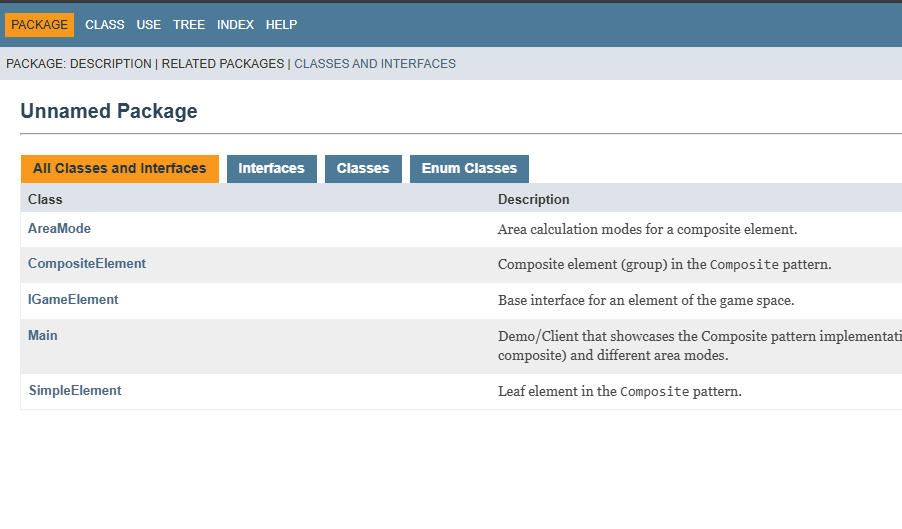
\includegraphics[width=0.9\textwidth]{demo1.png}
        % Підпис (зазвичай під малюнком):
        \caption{}

    \end{figure}

    \newpage

    \begin{center} \textbf{\Large Практична частина (Завдання №2)} \end{center}

    Номер залікової: $4106$, $4106 \text{ mod } 11 = 3$. Звідси завдання:

    \bigskip
    \begin{quote}
    Визначити специфiкацiї класiв, якi подають об'єкти-iконки для зображення елементiв
    файлової системи при побудовi графiчного iнтерфейсу користувача (GUI) – примiтиви
    (файли) та їх композицiї (директорiї). Забезпечити ефективне використання пам'ятi при
    роботi з великою кiлькiстю графiчних об'єктiв. Реалiзувати метод рисування графiчного
    об'єкту.
    \end{quote}
    \bigskip

    \setlength{\parindent}{1.5em}

    У цьому завданні використаю структурний шаблон проектування Flyweight (Легковаговик),
    який забезпечує ефективне використання пам'яті при роботі з великою кількістю графічних об'єктів (іконок файлів і директорій).
    Також частково застосовано Composite (Компонувальник) для побудови ієрархії елементів файлової системи.

    \vspace{0.6em}

    \setlength{\parindent}{0em}

    \textbf{\underline{Дерево робочої директорії до виконання \texttt{build}:}}

    \begin{minted}{text}
PS C:\Users\Artem Davydchuk\Desktop\reps\university_roadmap\semestr3\software engineering\labs\lab3\project2> tree /f /a 
Folder PATH listing
Volume serial number is 9873-FF92
C:.
|   build.xml
|
\---src
        DirectoryIcon.java
        FileIcon.java
        FSIcon.java
        IconFactory.java
        IconFlyweight.java
        IconType.java
        Main.jav
    \end{minted}

    \textbf{\underline{Код build.xml задля автоматизації:}}

    \begin{minted}{xml}
<?xml version="1.0" encoding="UTF-8"?>
<project name="lab3: Second Task" default="all" basedir=".">

  <!-- ===== Properties ===== -->
  <property name="src.dir"      value="src"/>
  <property name="build.dir"    value="out"/>
  <property name="classes.dir"  value="${build.dir}"/>
  <property name="doc.dir"      value="doc"/>
  <property name="main.class"   value="Main"/>
  <property name="java.release" value="17"/>

  <!-- ===== Clean ===== -->
  <target name="clean" description="Remove compiled classes and docs">
    <delete dir="${build.dir}"/>
    <delete dir="${doc.dir}"/>
  </target>

  <!-- ===== Compile ===== -->
  <target name="compile" description="Compile sources" depends="prepare">
    <mkdir dir="${classes.dir}"/>
    <javac srcdir="${src.dir}"
           destdir="${classes.dir}"
           includeantruntime="false"
           debug="true"
           encoding="UTF-8"
           release="${java.release}">
      <include name="**/*.java"/>
      <!-- Якщо з'явиться зовнішній classpath (JAR-и) — додай тут <classpath> -->
    </javac>
  </target>

  <target name="prepare">
    <mkdir dir="${classes.dir}"/>
  </target>

  <!-- ===== Run ===== -->
  <target name="run" description="Run main class" depends="compile">
    <java classname="${main.class}" fork="true" failonerror="true">
      <classpath>
        <path location="${classes.dir}"/>
      </classpath>
    </java>
  </target>

  <!-- ===== Javadoc ===== -->
  <target name="javadoc" description="Generate Javadoc">
    <mkdir dir="${doc.dir}"/>
    <javadoc destdir="${doc.dir}"
             sourcepath="${src.dir}"
             encoding="UTF-8"
             author="true"
             version="true"
             use="true"
             windowtitle="IPZ — API documentation"
             doctitle="IPZ — API documentation"
             failonerror="false">
      <fileset dir="${src.dir}">
        <include name="**/*.java"/>
      </fileset>
      <link href="https://docs.oracle.com/en/java/javase/${java.release}/docs/api/"/>
    </javadoc>
  </target>

  <!-- ===== All-in-one ===== -->
  <target name="all" description="Clean, compile, run, javadoc"
          depends="clean,compile,run,javadoc"/>
</project>
    \end{minted}

    \newpage

    \textbf{\underline{Команди (таски) які він виконує:}}

    \begin{minted}{text}
Buildfile: C:\Users\Artem Davydchuk\Desktop\reps\university_roadmap\semestr3\software engineering\labs\lab3\project2\build.xml

Main targets:

 all      Clean, compile, run, javadoc
 clean    Remove compiled classes and docs
 compile  Compile sources
 javadoc  Generate Javadoc
 run      Run main class
Default target: all
    \end{minted}

    \textbf{\underline{Результат виконання команди \texttt{all}:}}

    \begin{minted}{text}
PS C:\Users\Artem Davydchuk\Desktop\reps\university_roadmap\semestr3\software engineering\labs\lab3\project2> ant all 
Buildfile: C:\Users\Artem Davydchuk\Desktop\reps\university_roadmap\semestr3\software engineering\labs\lab3\project2\build.xml

clean:

prepare:
    [mkdir] Created dir: C:\Users\Artem Davydchuk\Desktop\reps\university_roadmap\semestr3\software engineering\labs\lab3\project2\out

compile:
    [javac] Compiling 7 source files to C:\Users\Artem Davydchuk\Desktop\reps\university_roadmap\semestr3\software engineering\labs\lab3\project2\out

run:
     [java] draw[FOLDER sprite=sprite-folder size=28x24] at=(10,10) label="root/"
     [java] draw[FILE sprite=sprite-file size=24x24] at=(10,40) label="README.md"
     [java] draw[FILE sprite=sprite-file size=24x24] at=(44,40) label=".gitignore"
     [java] draw[FOLDER sprite=sprite-folder size=28x24] at=(78,40) label="src/"
     [java] draw[FILE sprite=sprite-file size=24x24] at=(78,70) label="FSIcon.java"
     [java] draw[FILE sprite=sprite-file size=24x24] at=(112,70) label="IconFlyweight.java"
     [java] draw[FILE sprite=sprite-file size=24x24] at=(146,70) label="IconFactory.java"
     [java] draw[FILE sprite=sprite-file size=24x24] at=(180,70) label="FileIcon.java"
     [java] draw[FILE sprite=sprite-file size=24x24] at=(214,70) label="DirectoryIcon.java"
     [java] draw[FILE sprite=sprite-file size=24x24] at=(248,70) label="Main.java"
     [java] draw[FOLDER sprite=sprite-folder size=28x24] at=(112,40) label="doc/"
     [java] draw[FILE sprite=sprite-file size=24x24] at=(112,70) label="report.tex"
     [java] draw[FILE sprite=sprite-file size=24x24] at=(146,70) label="build.xml"
     [java] draw[FILE sprite=sprite-file size=24x24] at=(180,70) label="diagram.puml"
     [java]
     [java] Children in /src: 5006
     [java] Flyweights cached: 2 (should be 2: FILE and FOLDER)
     [java]
     [java] [Preview: redraw /src header only]
     [java] draw[FOLDER sprite=sprite-folder size=28x24] at=(10,200) label="src/"
     [java] ... (thousands of file icons share the same FILE flyweight)

javadoc:
    [mkdir] Created dir: C:\Users\Artem Davydchuk\Desktop\reps\university_roadmap\semestr3\software engineering\labs\lab3\project2\doc
  [javadoc] C:\Users\Artem Davydchuk\Desktop\reps\university_roadmap\semestr3\software engineering\labs\lab3\project2\src contains source files in the default package, you must specify them as source files not packages.
  [javadoc] Generating Javadoc
  [javadoc] Javadoc execution
  [javadoc] Loading source file C:\Users\Artem Davydchuk\Desktop\reps\university_roadmap\semestr3\software engineering\labs\lab3\project2\src\DirectoryIcon.java...
  [javadoc] Loading source file C:\Users\Artem Davydchuk\Desktop\reps\university_roadmap\semestr3\software engineering\labs\lab3\project2\src\FSIcon.java...
  [javadoc] Loading source file C:\Users\Artem Davydchuk\Desktop\reps\university_roadmap\semestr3\software engineering\labs\lab3\project2\src\FileIcon.java...
  [javadoc] Loading source file C:\Users\Artem Davydchuk\Desktop\reps\university_roadmap\semestr3\software engineering\labs\lab3\project2\src\IconFactory.java...
  [javadoc] Loading source file C:\Users\Artem Davydchuk\Desktop\reps\university_roadmap\semestr3\software engineering\labs\lab3\project2\src\IconFlyweight.java...
  [javadoc] Loading source file C:\Users\Artem Davydchuk\Desktop\reps\university_roadmap\semestr3\software engineering\labs\lab3\project2\src\IconType.java...
  [javadoc] Loading source file C:\Users\Artem Davydchuk\Desktop\reps\university_roadmap\semestr3\software engineering\labs\lab3\project2\src\Main.java...
  [javadoc] Constructing Javadoc information...
  [javadoc] Building index for all the packages and classes...
  [javadoc] Standard Doclet version 21.0.8+12-LTS-250
  [javadoc] Building tree for all the packages and classes...
  [javadoc] C:\Users\Artem Davydchuk\Desktop\reps\university_roadmap\semestr3\software engineering\labs\lab3\project2\src\FileIcon.java:4: error: bad HTML entity
  [javadoc]  * Extrinsic state: file name, local position; intrinsic: shared sprite & size.
  [javadoc]                                                                         ^
  [javadoc] Generating C:\Users\Artem Davydchuk\Desktop\reps\university_roadmap\semestr3\software engineering\labs\lab3\project2\doc\DirectoryIcon.html...
  [javadoc] C:\Users\Artem Davydchuk\Desktop\reps\university_roadmap\semestr3\software engineering\labs\lab3\project2\src\FSIcon.java:7: warning: no main description
  [javadoc]     /** @return display name (file or directory name) */
  [javadoc]         ^
  [javadoc] C:\Users\Artem Davydchuk\Desktop\reps\university_roadmap\semestr3\software engineering\labs\lab3\project2\src\FSIcon.java:11: warning: no @return
  [javadoc]     int getX();
  [javadoc]         ^
  [javadoc] C:\Users\Artem Davydchuk\Desktop\reps\university_roadmap\semestr3\software engineering\labs\lab3\project2\src\FSIcon.java:16: warning: no @return
  [javadoc]     int getWidth();
  [javadoc]         ^
  [javadoc] C:\Users\Artem Davydchuk\Desktop\reps\university_roadmap\semestr3\software engineering\labs\lab3\project2\src\DirectoryIcon.java:27: warning: no @param for child
  [javadoc]     public void add(FSIcon child) {
  [javadoc]                 ^
  [javadoc] C:\Users\Artem Davydchuk\Desktop\reps\university_roadmap\semestr3\software engineering\labs\lab3\project2\src\DirectoryIcon.java:41: warning: no @param for child
  [javadoc]     public void remove(FSIcon child) { children.remove(child); }
  [javadoc]                 ^
  [javadoc] C:\Users\Artem Davydchuk\Desktop\reps\university_roadmap\semestr3\software engineering\labs\lab3\project2\src\DirectoryIcon.java:43: warning: no main description
  [javadoc]     /** @return immutable view of children */
  [javadoc]         ^
  [javadoc] C:\Users\Artem Davydchuk\Desktop\reps\university_roadmap\semestr3\software engineering\labs\lab3\project2\src\DirectoryIcon.java:47: warning: no @param for columns
  [javadoc]     public DirectoryIcon setGrid(int columns, int hGap, int vGap) {
  [javadoc]                          ^
  [javadoc] C:\Users\Artem Davydchuk\Desktop\reps\university_roadmap\semestr3\software engineering\labs\lab3\project2\src\DirectoryIcon.java:47: warning: no @param for hGap
  [javadoc]     public DirectoryIcon setGrid(int columns, int hGap, int vGap) {
  [javadoc]                          ^
  [javadoc] C:\Users\Artem Davydchuk\Desktop\reps\university_roadmap\semestr3\software engineering\labs\lab3\project2\src\DirectoryIcon.java:47: warning: no @param for vGap
  [javadoc]     public DirectoryIcon setGrid(int columns, int hGap, int vGap) {
  [javadoc]                          ^
  [javadoc] C:\Users\Artem Davydchuk\Desktop\reps\university_roadmap\semestr3\software engineering\labs\lab3\project2\src\DirectoryIcon.java:47: warning: no @return
  [javadoc]     public DirectoryIcon setGrid(int columns, int hGap, int vGap) {
  [javadoc]                          ^
  [javadoc] C:\Users\Artem Davydchuk\Desktop\reps\university_roadmap\semestr3\software engineering\labs\lab3\project2\src\DirectoryIcon.java:21: warning: no comment
  [javadoc]     public DirectoryIcon(String dirName) {
  [javadoc]            ^
  [javadoc] C:\Users\Artem Davydchuk\Desktop\reps\university_roadmap\semestr3\software engineering\labs\lab3\project2\src\FSIcon.java:12: warning: no comment
  [javadoc]     int getY();
  [javadoc]         ^
  [javadoc] C:\Users\Artem Davydchuk\Desktop\reps\university_roadmap\semestr3\software engineering\labs\lab3\project2\src\FSIcon.java:13: warning: no comment
  [javadoc]     void setPosition(int x, int y);
  [javadoc]          ^
  [javadoc] C:\Users\Artem Davydchuk\Desktop\reps\university_roadmap\semestr3\software engineering\labs\lab3\project2\src\FSIcon.java:17: warning: no comment
  [javadoc]     int getHeight();
  [javadoc]         ^
  [javadoc] Generating C:\Users\Artem Davydchuk\Desktop\reps\university_roadmap\semestr3\software engineering\labs\lab3\project2\doc\FileIcon.html...
  [javadoc] Generating C:\Users\Artem Davydchuk\Desktop\reps\university_roadmap\semestr3\software engineering\labs\lab3\project2\doc\FSIcon.html...
  [javadoc] Generating C:\Users\Artem Davydchuk\Desktop\reps\university_roadmap\semestr3\software engineering\labs\lab3\project2\doc\IconFactory.html...
  [javadoc] C:\Users\Artem Davydchuk\Desktop\reps\university_roadmap\semestr3\software engineering\labs\lab3\project2\src\IconFactory.java:14: warning: no @param for type
  [javadoc]     public static IconFlyweight get(IconType type) {
  [javadoc]                                 ^
  [javadoc] C:\Users\Artem Davydchuk\Desktop\reps\university_roadmap\semestr3\software engineering\labs\lab3\project2\src\IconFactory.java:14: warning: no @return
  [javadoc]     public static IconFlyweight get(IconType type) {
  [javadoc]                                 ^
  [javadoc] C:\Users\Artem Davydchuk\Desktop\reps\university_roadmap\semestr3\software engineering\labs\lab3\project2\src\IconFactory.java:27: warning: no main description
  [javadoc]     /** @return how many flyweights are currently cached (should be small). */
  [javadoc]         ^
  [javadoc] Generating C:\Users\Artem Davydchuk\Desktop\reps\university_roadmap\semestr3\software engineering\labs\lab3\project2\doc\IconFlyweight.html...
  [javadoc] C:\Users\Artem Davydchuk\Desktop\reps\university_roadmap\semestr3\software engineering\labs\lab3\project2\src\IconFlyweight.java:18: warning: no main description
  [javadoc]     /** @return icon type (FILE/FOLDER) */
  [javadoc]         ^
  [javadoc] C:\Users\Artem Davydchuk\Desktop\reps\university_roadmap\semestr3\software engineering\labs\lab3\project2\src\IconFlyweight.java:21: warning: no main description
  [javadoc]     /** @return logical sprite identifier (e.g., resource name) */
  [javadoc]         ^
  [javadoc] C:\Users\Artem Davydchuk\Desktop\reps\university_roadmap\semestr3\software engineering\labs\lab3\project2\src\IconFlyweight.java:24: warning: no main description
  [javadoc]     /** @return intrinsic width */
  [javadoc]         ^
  [javadoc] C:\Users\Artem Davydchuk\Desktop\reps\university_roadmap\semestr3\software engineering\labs\lab3\project2\src\IconFlyweight.java:27: warning: no main description
  [javadoc]     /** @return intrinsic height */
  [javadoc]         ^
  [javadoc] C:\Users\Artem Davydchuk\Desktop\reps\university_roadmap\semestr3\software engineering\labs\lab3\project2\src\IconFlyweight.java:34: warning: no @param for label
  [javadoc]     public void paint(String label, int absX, int absY) {
  [javadoc]                 ^
  [javadoc] C:\Users\Artem Davydchuk\Desktop\reps\university_roadmap\semestr3\software engineering\labs\lab3\project2\src\IconFlyweight.java:34: warning: no @param for absX
  [javadoc]     public void paint(String label, int absX, int absY) {
  [javadoc]                 ^
  [javadoc] C:\Users\Artem Davydchuk\Desktop\reps\university_roadmap\semestr3\software engineering\labs\lab3\project2\src\IconFlyweight.java:34: warning: no @param for absY
  [javadoc]     public void paint(String label, int absX, int absY) {
  [javadoc]                 ^
  [javadoc] C:\Users\Artem Davydchuk\Desktop\reps\university_roadmap\semestr3\software engineering\labs\lab3\project2\src\IconFlyweight.java:11: warning: no comment
  [javadoc]     public IconFlyweight(IconType type, String spriteName, int width, int height) {
  [javadoc]            ^
  [javadoc] Generating C:\Users\Artem Davydchuk\Desktop\reps\university_roadmap\semestr3\software engineering\labs\lab3\project2\doc\IconType.html...
  [javadoc] C:\Users\Artem Davydchuk\Desktop\reps\university_roadmap\semestr3\software engineering\labs\lab3\project2\src\IconType.java:3: warning: no comment
  [javadoc]     FILE,
  [javadoc]     ^
  [javadoc] C:\Users\Artem Davydchuk\Desktop\reps\university_roadmap\semestr3\software engineering\labs\lab3\project2\src\IconType.java:4: warning: no comment
  [javadoc]     FOLDER
  [javadoc]     ^
  [javadoc] Generating C:\Users\Artem Davydchuk\Desktop\reps\university_roadmap\semestr3\software engineering\labs\lab3\project2\doc\Main.html...
  [javadoc] C:\Users\Artem Davydchuk\Desktop\reps\university_roadmap\semestr3\software engineering\labs\lab3\project2\src\Main.java:5: warning: use of default constructor, which does not provide a comment
  [javadoc] public class Main {
  [javadoc]        ^
  [javadoc] C:\Users\Artem Davydchuk\Desktop\reps\university_roadmap\semestr3\software engineering\labs\lab3\project2\src\Main.java:6: warning: no comment
  [javadoc]     public static void main(String[] args) {
  [javadoc]                        ^
  [javadoc] Generating C:\Users\Artem Davydchuk\Desktop\reps\university_roadmap\semestr3\software engineering\labs\lab3\project2\doc\package-summary.html...
  [javadoc] Generating C:\Users\Artem Davydchuk\Desktop\reps\university_roadmap\semestr3\software engineering\labs\lab3\project2\doc\package-tree.html...
  [javadoc] Generating C:\Users\Artem Davydchuk\Desktop\reps\university_roadmap\semestr3\software engineering\labs\lab3\project2\doc\class-use\DirectoryIcon.html...
  [javadoc] Generating C:\Users\Artem Davydchuk\Desktop\reps\university_roadmap\semestr3\software engineering\labs\lab3\project2\doc\class-use\FSIcon.html...
  [javadoc] Generating C:\Users\Artem Davydchuk\Desktop\reps\university_roadmap\semestr3\software engineering\labs\lab3\project2\doc\class-use\FileIcon.html...
  [javadoc] Generating C:\Users\Artem Davydchuk\Desktop\reps\university_roadmap\semestr3\software engineering\labs\lab3\project2\doc\class-use\IconFactory.html...
  [javadoc] Generating C:\Users\Artem Davydchuk\Desktop\reps\university_roadmap\semestr3\software engineering\labs\lab3\project2\doc\class-use\IconFlyweight.html...
  [javadoc] Generating C:\Users\Artem Davydchuk\Desktop\reps\university_roadmap\semestr3\software engineering\labs\lab3\project2\doc\class-use\IconType.html...
  [javadoc] Generating C:\Users\Artem Davydchuk\Desktop\reps\university_roadmap\semestr3\software engineering\labs\lab3\project2\doc\class-use\Main.html...
  [javadoc] Generating C:\Users\Artem Davydchuk\Desktop\reps\university_roadmap\semestr3\software engineering\labs\lab3\project2\doc\package-use.html...
  [javadoc] Generating C:\Users\Artem Davydchuk\Desktop\reps\university_roadmap\semestr3\software engineering\labs\lab3\project2\doc\overview-tree.html...
  [javadoc] Building index for all classes...
  [javadoc] Generating C:\Users\Artem Davydchuk\Desktop\reps\university_roadmap\semestr3\software engineering\labs\lab3\project2\doc\allclasses-index.html...
  [javadoc] Generating C:\Users\Artem Davydchuk\Desktop\reps\university_roadmap\semestr3\software engineering\labs\lab3\project2\doc\allpackages-index.html...
  [javadoc] Generating C:\Users\Artem Davydchuk\Desktop\reps\university_roadmap\semestr3\software engineering\labs\lab3\project2\doc\index-all.html...
  [javadoc] Generating C:\Users\Artem Davydchuk\Desktop\reps\university_roadmap\semestr3\software engineering\labs\lab3\project2\doc\search.html...
  [javadoc] Generating C:\Users\Artem Davydchuk\Desktop\reps\university_roadmap\semestr3\software engineering\labs\lab3\project2\doc\index.html...
  [javadoc] Generating C:\Users\Artem Davydchuk\Desktop\reps\university_roadmap\semestr3\software engineering\labs\lab3\project2\doc\help-doc.html...
  [javadoc] 1 error
  [javadoc] 29 warnings

all:

BUILD SUCCESSFUL
Total time: 5 seconds
    \end{minted}

    \textbf{\underline{Оновлене дерево робочої директорії:}}

    \begin{minted}{text}
PS C:\Users\Artem Davydchuk\Desktop\reps\university_roadmap\semestr3\software engineering\labs\lab3\project2> tree /f /a
Folder PATH listing
Volume serial number is 9873-FF92
C:.
|   build.xml
|
+---doc
|   |   allclasses-index.html
|   |   allpackages-index.html
|   |   copy.svg
|   |   DirectoryIcon.html
|   |   element-list
|   |   FileIcon.html
|   |   FSIcon.html
|   |   help-doc.html
|   |   IconFactory.html
|   |   IconFlyweight.html
|   |   IconType.html
|   |   index-all.html
|   |   index.html
|   |   link.svg
|   |   Main.html
|   |   member-search-index.js
|   |   module-search-index.js
|   |   overview-tree.html
|   |   package-search-index.js
|   |   package-summary.html
|   |   package-tree.html
|   |   package-use.html
|   |   script.js
|   |   search-page.js
|   |   search.html
|   |   search.js
|   |   stylesheet.css
|   |   tag-search-index.js
|   |   type-search-index.js
|   |
|   +---class-use
|   |       DirectoryIcon.html
|   |       FileIcon.html
|   |       FSIcon.html
|   |       IconFactory.html
|   |       IconFlyweight.html
|   |       IconType.html
|   |       Main.html
|   |
|   +---legal
|   |       COPYRIGHT
|   |       jquery.md
|   |       jqueryUI.md
|   |       LICENSE
|   |
|   +---resources
|   |       glass.png
|   |       x.png
|   |
|   \---script-dir
|           jquery-3.7.1.min.js
|           jquery-ui.min.css
|           jquery-ui.min.js
|
+---out
|       DirectoryIcon.class
|       FileIcon.class
|       FSIcon.class
|       IconFactory$1.class
|       IconFactory.class
|       IconFlyweight.class
|       IconType.class
|       Main.class
|
\---src
        DirectoryIcon.java
        FileIcon.java
        FSIcon.java
        IconFactory.java
        IconFlyweight.java
        IconType.java
        Main.java
    \end{minted}

    \textbf{\underline{Додатковий окремий запуск Main:}}

    \begin{minted}{text}
PS C:\Users\Artem Davydchuk\Desktop\reps\university_roadmap\semestr3\software engineering\labs\lab3\project2> java -cp out Main
draw[FOLDER sprite=sprite-folder size=28x24] at=(10,10) label="root/"
draw[FILE sprite=sprite-file size=24x24] at=(10,40) label="README.md"
draw[FILE sprite=sprite-file size=24x24] at=(44,40) label=".gitignore"
draw[FOLDER sprite=sprite-folder size=28x24] at=(78,40) label="src/"
draw[FILE sprite=sprite-file size=24x24] at=(78,70) label="FSIcon.java"
draw[FILE sprite=sprite-file size=24x24] at=(112,70) label="IconFlyweight.java"
draw[FILE sprite=sprite-file size=24x24] at=(146,70) label="IconFactory.java"
draw[FILE sprite=sprite-file size=24x24] at=(180,70) label="FileIcon.java"
draw[FILE sprite=sprite-file size=24x24] at=(214,70) label="DirectoryIcon.java"
draw[FILE sprite=sprite-file size=24x24] at=(248,70) label="Main.java"
draw[FOLDER sprite=sprite-folder size=28x24] at=(112,40) label="doc/"
draw[FILE sprite=sprite-file size=24x24] at=(112,70) label="report.tex"
draw[FILE sprite=sprite-file size=24x24] at=(146,70) label="build.xml"
draw[FILE sprite=sprite-file size=24x24] at=(180,70) label="diagram.puml"

Children in /src: 5006
Flyweights cached: 2 (should be 2: FILE and FOLDER)

[Preview: redraw /src header only]
draw[FOLDER sprite=sprite-folder size=28x24] at=(10,200) label="src/"
... (thousands of file icons share the same FILE flyweight)
    \end{minted}

    Відкриваємо \texttt{index.html} у браузері:

    \begin{figure}[h!]

        \renewcommand{\thefigure}{\arabic{figure}} % робимо "3.1", "3.2" і т.д.

        \centering
        % Підставляєте потрібний шлях та розмір зображення:
        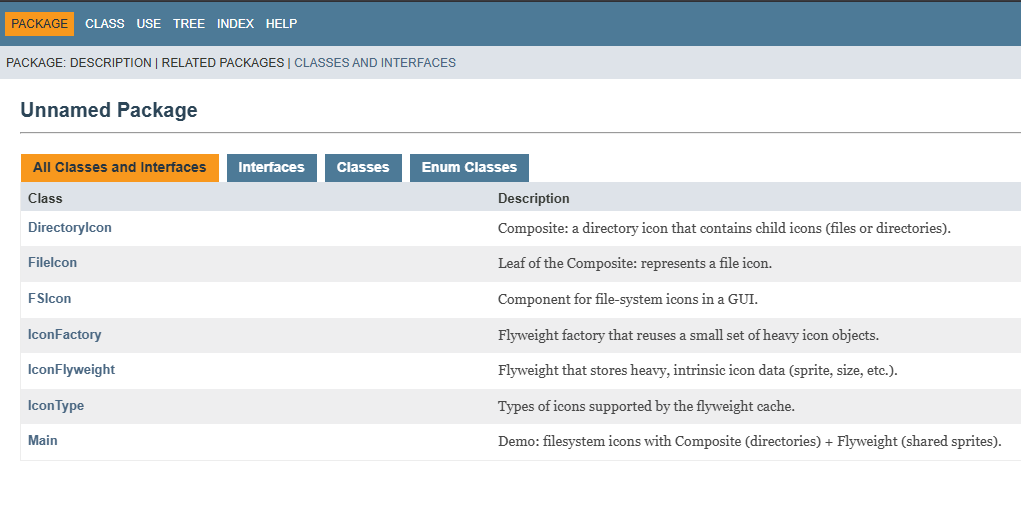
\includegraphics[width=0.9\textwidth]{demo2.png}
        % Підпис (зазвичай під малюнком):
        \caption{}

    \end{figure}

    \newpage

    \textbf{\underline{Висновок:}} У результаті виконання лабораторної роботи було розроблено програмну модель,
яка відображає елементи файлової системи у вигляді графічних іконок.
Під час реалізації було використано структурні шаблони проектування
\textbf{Flyweight (Легковаговик)} та \textbf{Composite (Компонувальник)}.

\setlength{\parindent}{1.5em}

Застосування шаблону \textbf{Flyweight} забезпечило ефективне використання
пам'яті завдяки спільному зберіганню важких графічних ресурсів (іконок),
які використовуються численними об’єктами файлової системи.
Кожен об’єкт має власний зовнішній стан (ім’я, координати розташування),
але спільно використовує внутрішній стан — графічне зображення, розміри та тип піктограми.

Шаблон \textbf{Composite} дозволив реалізувати ієрархічну структуру файлової системи,
де директорії можуть містити як окремі файли, так і інші вкладені директорії.
Це забезпечило уніфіковану роботу з усіма об’єктами через спільний інтерфейс
та спростило виконання операцій відображення.

Таким чином, поставлене завдання виконано: створено систему класів, яка
забезпечує ефективну обробку та відображення великої кількості графічних об’єктів
із мінімальними витратами пам’яті.

\end{document}